\section{Sensemaking with SchemaLine}
\label{sec:interaction}

%We first discuss about the visual encoding of events and schemata; and then how sense making activities in Data-Frame model are supported in SchemaLine.

%\subsection{Event and Schema Representation}
%\label{sub:visual-encoding}
%\paragraph*{Event Representation}
%%Appearance
%An event is represented by a rounded rectangle with its left side aligned with the event's time on the timeline. To reduce cluttering, events are not constantly connected by lines to their corresponding points on the timeline. Instead, when the mouse is over an event, its time point on the timeline is highlighted. A short text is rendered inside the rectangle to summarize the event. To address the scalability of long texts, we assign a maximum width to event rectangles and trim exceeding texts. The full content will only be displayed when the note is hovered over. All events have a uniform height to give a nice overall appearance, especially when they are connected to form a schema (Section \ref{sub:schema-outline}). Quite often, events are categorical data. For example, in news reports, an article can be classified into sport, fashion or both. SchemaLine adds a small rectangle in each event to color-code its categorization. Eight different colors are supported, which are chosen from qualitative colors -- Set 1 of ColorBrewer \cite{Harrower2003}. All other categories besides eight of the most popular ones will share the same color to address the limitation of small distinguishable colors. We plan to combine colors with other indicators such as texture to increase the number of differentiated keywords in the future work. The number of maximum categories that an event can belong to is configurable to adapt the dataset characteristics. As in Fig.~\ref{fig:notes-only}, maximum four themes of an event can be displayed.
%
%\begin{figure}[ht]
%\centering
%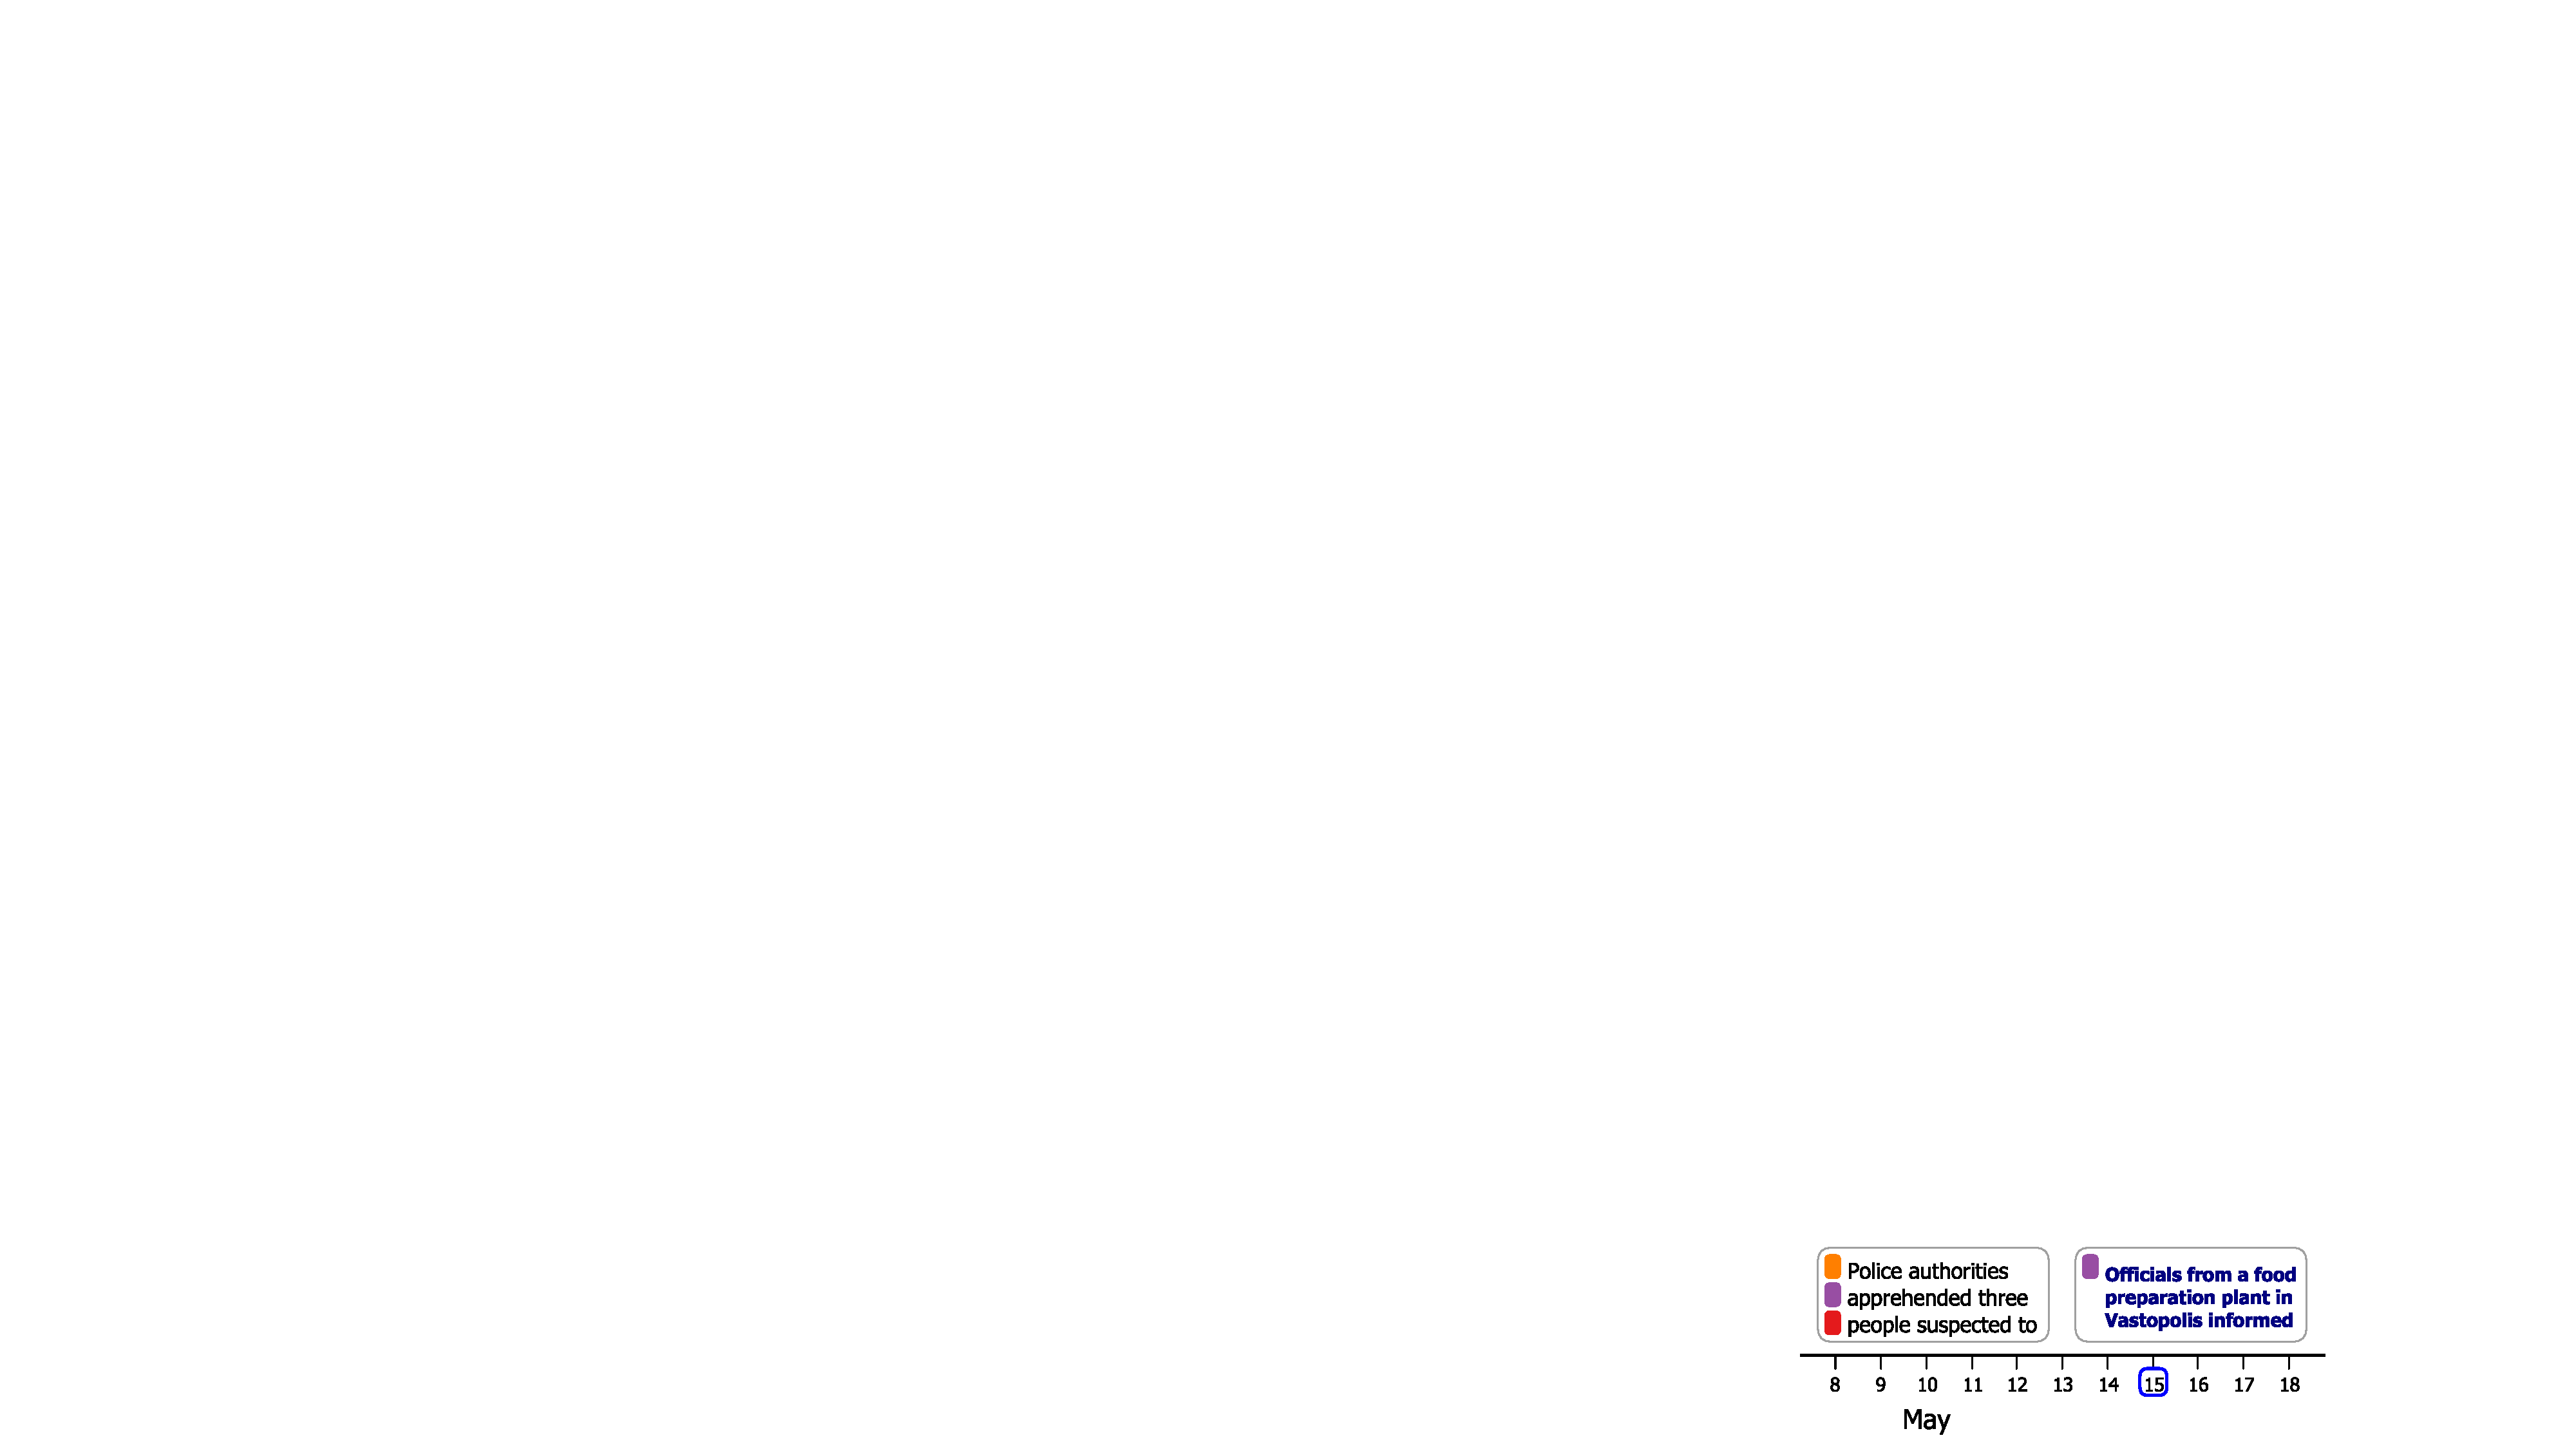
\includegraphics[width=\linewidth]{notes-only}
%\caption{Bigger texts, two events are ok, no need change time. Events are represented by rounded rectangles with uniform height and limited widths for displaying texts. On the left side of the event rectangle, there are some small color-coded rectangles to represent the event's themes.}
%\label{fig:notes-only}
%\end{figure}
%
%%Timeline appearance
%In SchemaLine, the timeline is shown as a horizontal axis at the bottom of the display. Its starting and ending points change dynamically to cover the time span of all events. The timeline consists of two temporal scales. These two scales can also be changed dynamically according to the displayed events. For example, they change from ``month/day'' to ``year/month'' to accommodate large interval increases.
%
%\paragraph*{Schema Representation}
%After discovering a number of relevant events or evidence, the analyst starts combining them to form a \textit{schema}. A schema is a set of related events that are connected to each other in a certain way. For example, a schema can contain all events about a particular person. Multiple schemata can be composed in SchemaLine as shown in Fig.~\ref{fig:teaser}. 
%
%We consider several design options to connect events within a schema such as using colors~\cite{TimeGlider2013} or node-link diagram~\cite{Jensen2003}. However, they all have some drawbacks as discussed in the Related work (Section~\ref{sec:relatedwork}). Computational methods that allow visualize a large number of events with different themes such as ThemeRiver~\cite{Havre2002} do not work either because individual events and interactions are more essential in SchemaLine. Also, it should be easy to follow events within a schema in temporal order. We decided to visualize each schema as a colored stripe, which is inspired by Munroe's hand-drawn visualization~\cite{Munroe2009}. A character line in Munroe's work connects all events happened to that character. Similarly, our schema is a color stripe connecting all events belonging to it. Instead of using a thin line, we use a path with unique width (an event's height) to make enough space for displaying the event's summary text and possible to interact with individual notes. A rectilinear path is employed to provide a nice visualization rather than direct connection between events. An example can be seen in Fig.~\ref{fig:schema} and details of the algorithm to generate the schema layout and outline will be discussed in Section~\ref{sec:layout}.
%\begin{figure}[ht]
%\centering
%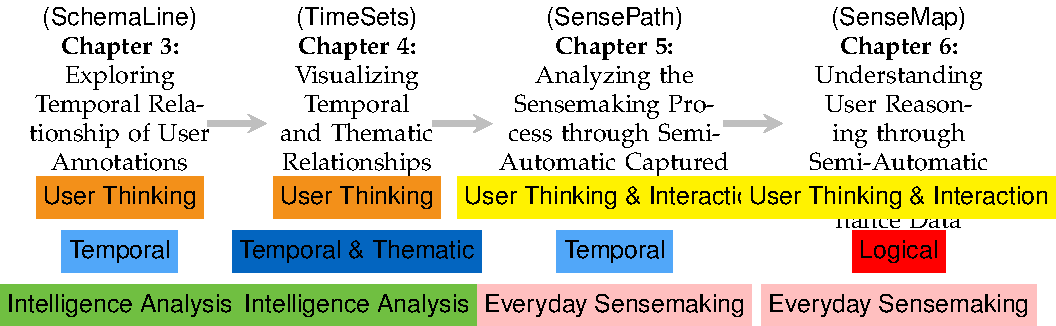
\includegraphics[width=\linewidth]{story}
%\caption{A schema with rounded corners.}
%\label{fig:schema}
%\end{figure}

%In the SchemaLine, each white rectangle is an analysis note, linking to the document in the search results that led to this discovery and positioned along the time axis at the point when the event happened. Notes can be grouped together to form a ``story''. There are three stories in this example and they are in red, blue, and orange. In the middle are the results of two searches: ``vastopolis'' and ``terrorist''. At the very top is a list of minimized searches, only showing the keywords. 


%Pirolli and Card~\cite{Pirolli2005} regarded the timeline as an effective tool for the ``Schematize'' task. A timeline can not only reveal the temporal relationships among the findings, but also have a considerable impact on how easily they can be understood. Pennington and Hastie~\cite{Pennington1991} studied the impact of evidence presentation order on juror decision making. They found that information was easier to understand when presented in chronological order and thus had a significant impact on jurors' decisions. 

%\subsection{Sensemaking with Data-Frame Model}
%\label{sub:interactive-editing}
SchemaLine is designed to support all five sensemaking activities in Data-Frame model through fluid user interactions. Following the design guidelines for fluidity proposed by Elmqvist et al.~\cite{Elmqvist2011}, SchemaLine's interactions
\begin{itemize}
	\item use smooth animated transitions between states,
	\item provide immediate visual feedback on interaction, and
	\item use direct manipulation of visual representations.
\end{itemize}

Sensemaking activities in Data-Frame model involve two different types of entities: \textit{data} and \textit{frame}. We allow direct manipulation of visual representations of data and frame, instead of invoking menus and buttons to perform actions. The first sensemaking activity in the Data-Frame model is to \textbf{construct a new frame} by connecting relevant data. It can be performed in SchemaLine by \textit{dragging one event and dropping it onto another event}. A \textit{plus} icon and a \textit{dashed rectangle} surrounding the two events are displayed to indicate that a new frame will be created. When dropping the event, a color stripe representing a frame will be formed by connecting these two events, and a smooth animated transition is used to improve user perception.

Besides dropping an event on top of another event, the user can drop it onto the color stripe to add that event to an existing frame (\textbf{elaborate a frame}). Conversely, the user can drag an event belonging to a frame and drop it onto the void space to remove it from the frame (\textbf{preserving a frame}). Appropriate informative feedback is displayed, \textit{plus} icon for addition and \textit{minus} icon for subtraction, and a smooth animated transition is used to improve user perception. Fig.~\ref{fig:drag-drop-note} shows an example of adding an event into a frame.
\begin{figure}[ht]
\centering
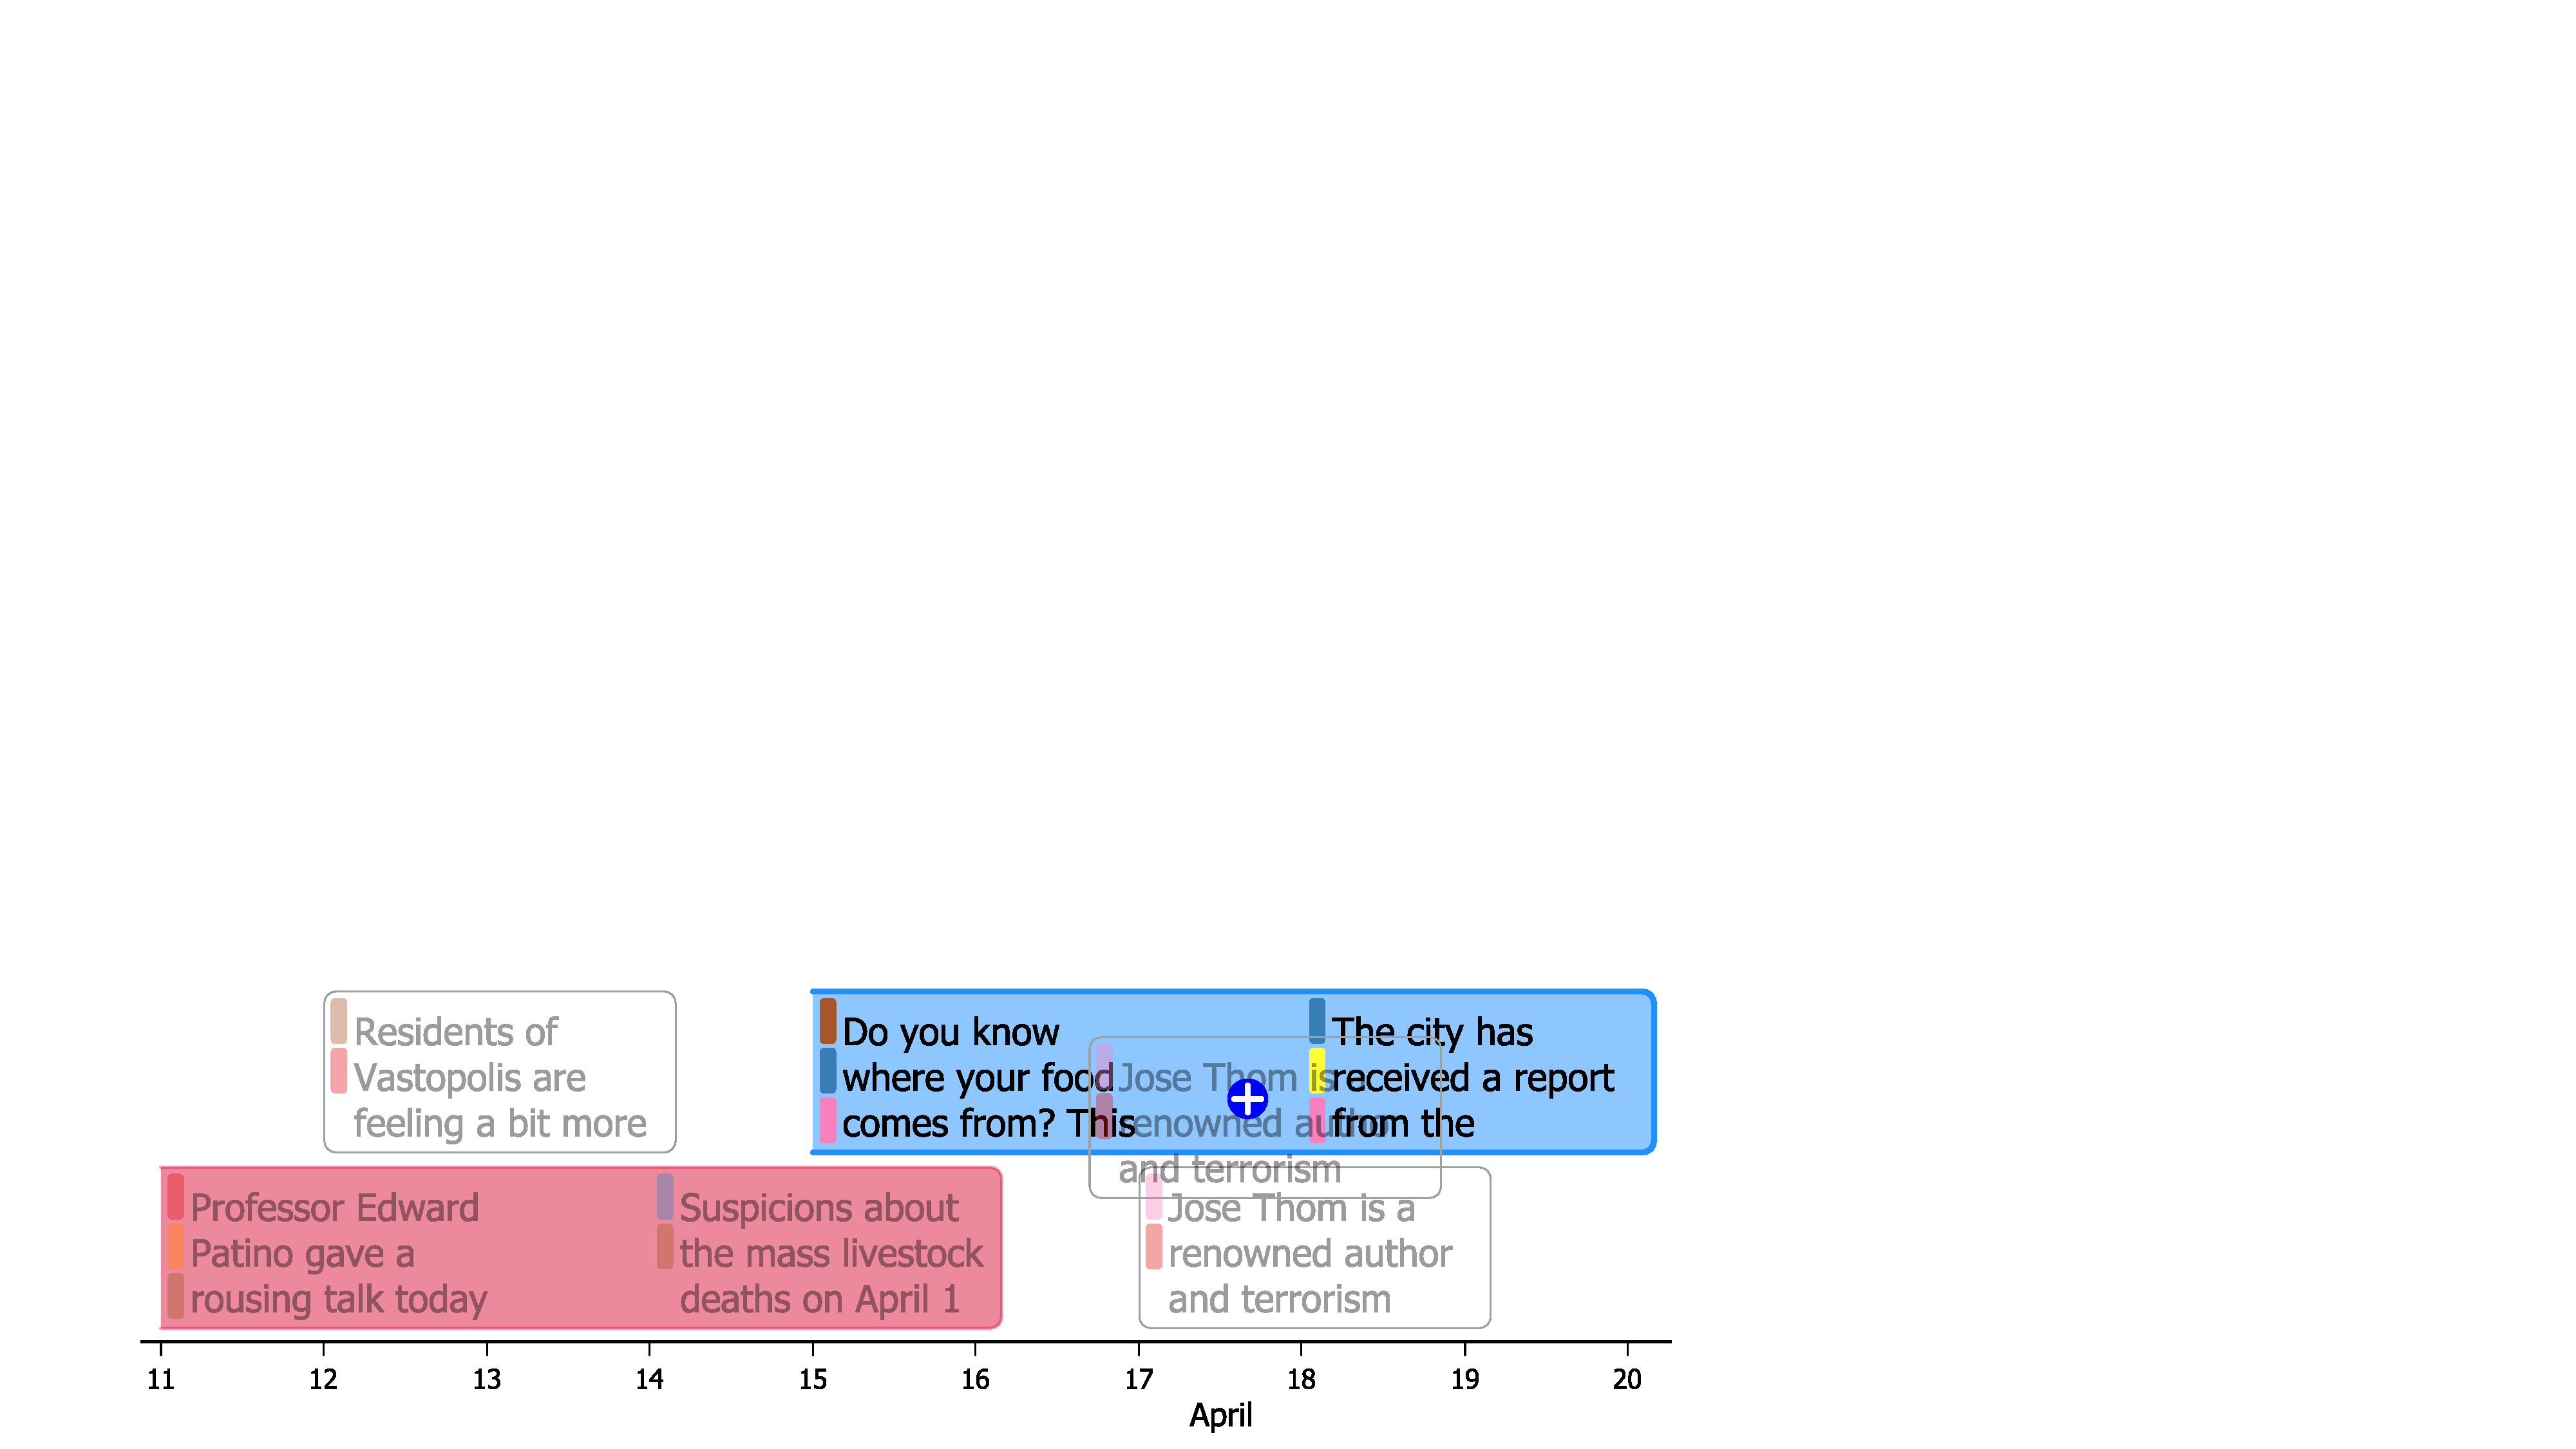
\includegraphics[width=\linewidth]{add-event-frame}
\caption{Each frame is represented as a colored stripe. Dropping an event onto the blue stripe means adding that event into the blue frame to elaborate it.}
\label{fig:drag-drop-note}
\end{figure}

\textbf{Questioning a frame} occurs when the user encounters inconsistencies in data within a frame. The temporal distribution of events in the frame may suggest some concerns about the validity or completeness of the frame. For example, if a frame about one person contains many events in January and March, but no events are found in February, then it may be inferred that there could be some data missing. The analyst can mark a suspected event by right-mouse double-clicking on it. Red color text is used to indicate that the event needs more investigation. 

Dragging an event from one frame to another frame will remove it from the old frame and add it to the new frame. However, holding \textit{Control} key when dropping will instead copy the event to the new frame. This interaction allows the analyst to duplicate events to create several similar frames and compare them (\textbf{comparing frames}). When two frames are selected, they will be moved closer together to allow easy comparison, irrespective of the frames ordering generated by the layout algorithm. The user can drag an entire frame and drop it onto another frame to merge all events together. The user can also drop the frame onto the void space to take apart the frame and release its events. This interaction is useful when the user thinks that the frame is completely wrong and wants to construct a new frame (\textbf{reframing}).

Other interactions with events are also designed to be intuitive. Left-mouse double-clicking on an event opens its full content. Dragging an event with the right mouse button can change the event's date. This feature is useful because the report date is not always the date when the event actually occurred; for example, ``yesterday there was a bomb attack in ABC''. Dragging an event outside the boundary of the timeline will remove it from the system (with \textit{remove} icon as informative feedback).

Once any change is made on SchemaLine, such as moving an event from one frame to another, an animation is shown of smooth transition between the changes to help analyst update their ``mental map''. To achieve this, the layout algorithm (Section \ref{sub:schema-layout}) computes the new event rectangle locations. Then, the outline algorithm (Section \ref{sub:schema-outline}) runs at every step of the interpolation between the old and the new locations to produce intermediate polygon paths based on the updated event locations.